\documentclass[tikz]{standalone}
\usepackage{geometricfigures}

\usepackage{xcolor}
\usepackage{pgfplots}
\pgfplotsset{compat=1.18}
\usetikzlibrary{calc}

\begin{document}
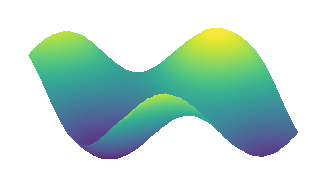
\begin{tikzpicture}[
                scale=0.5,
                arrow/.style={->, >=Stealth, thick},
            ]
                \begin{axis}[
                view={-30}{30}, % Adjust the view for better visibility
                colormap/viridis, % Use the viridis colormap
                hide axis,
            ]
                % (ii) Plot the 2D manifold with the Julia-like (viridis) colormap
                \addplot3[
                    surf,
                    shader=interp,
                    domain=-5:5,
                    y domain=-5:5,
                    samples=50,
                    opacity=0.9,
                    axis line style={draw=none},
                    tick style={draw=none},
                ]{sin(deg(.5*x)) * cos(deg(.5*y))};
                
            \end{axis}
\end{tikzpicture}
\end{document}
